\section{Live Demo}
    
    \frame{\sectionpage}
    
    \begin{frame}{Robot Nao 6 Database}
    	\begin{figure}
    		\centering
    		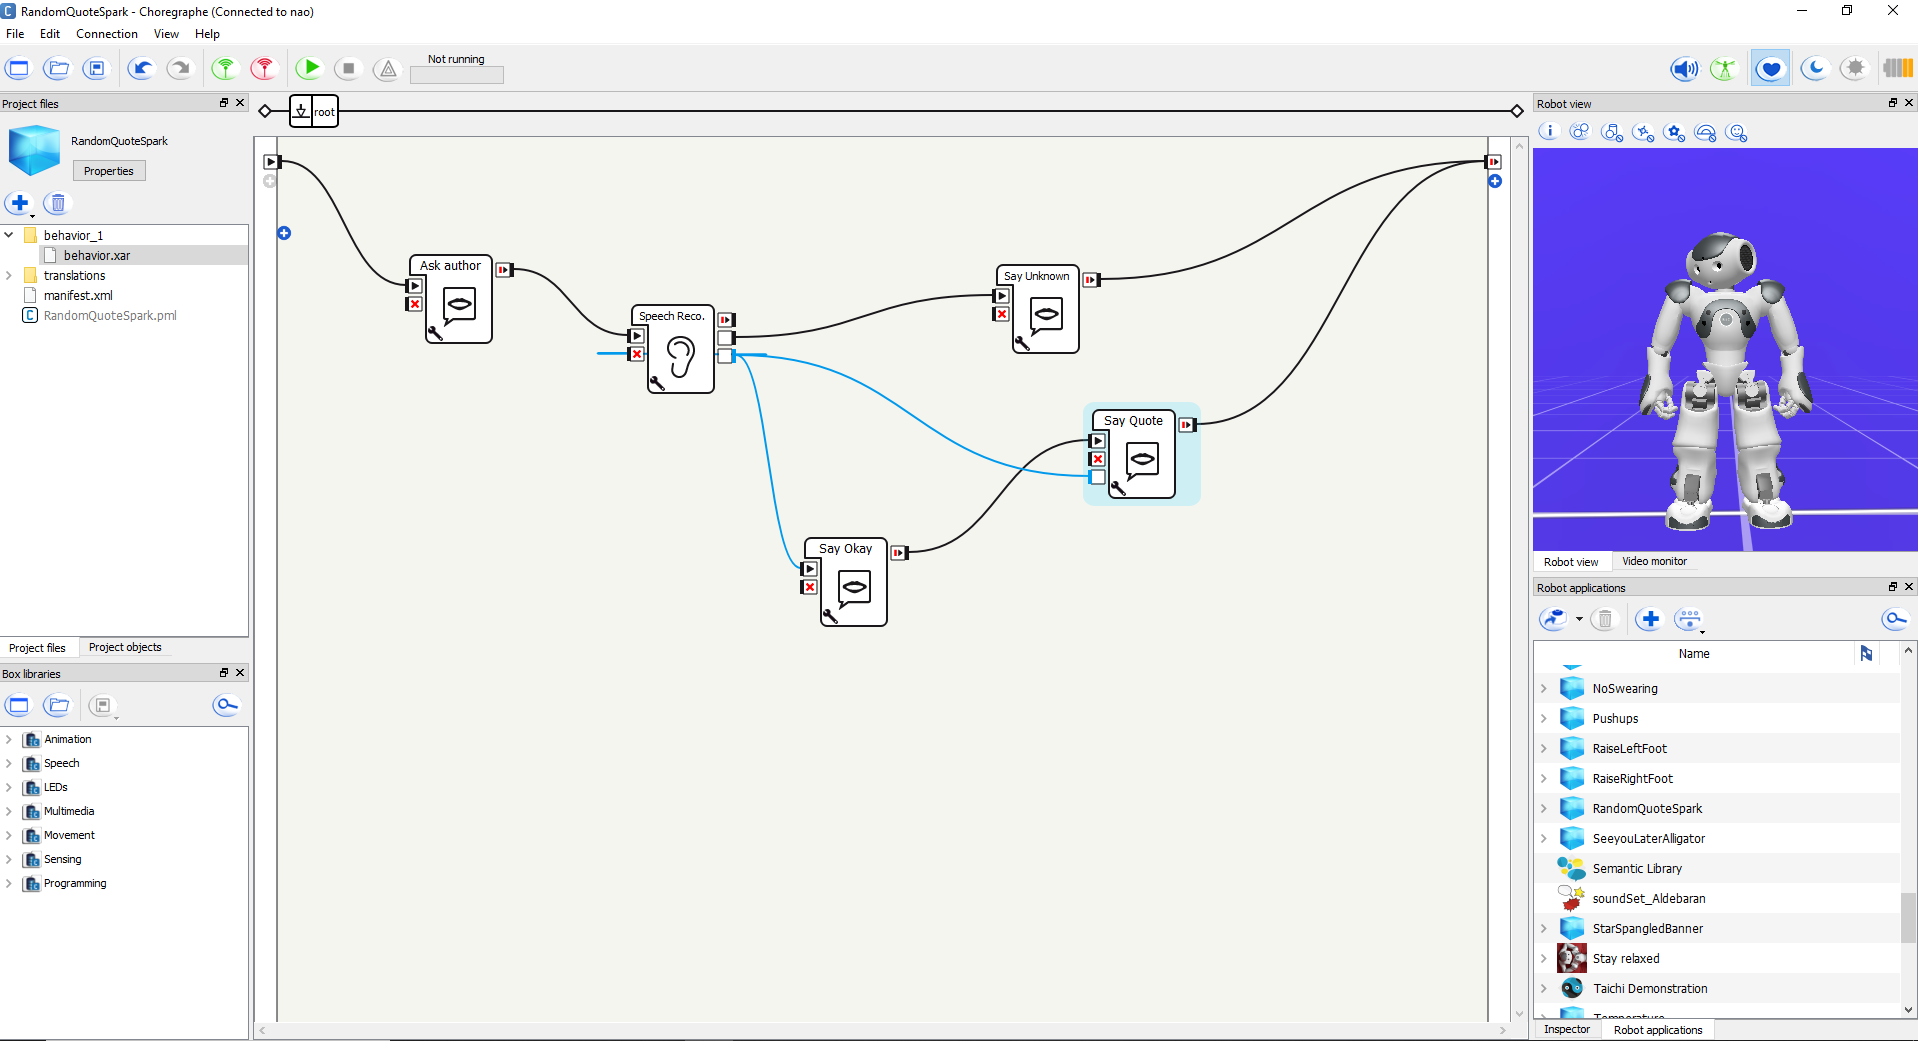
\includegraphics[width =1\linewidth]{robot-spark-proj/screenshot-1.PNG}
    		\caption{Diagram}
    	\end{figure}
    	
    \end{frame}
	{Python2 code with robot}
	\begin{verbatim}
	import time
	import requests
	
	author = ""
	
	class MyClass(GeneratedClass):
	def __init__(self):
	GeneratedClass.__init__(self, False)
	
	def onLoad(self):
	self.tts = self.session().service('ALTextToSpeech')
	self.ttsStop = self.session().service('ALTextToSpeech') #Create another service as wait is blocking if audioout is remote
	self.bIsRunning = False
	self.ids = []
	
	def onUnload(self):
	for id in self.ids:
	try:
	self.ttsStop.stop(id)
	except:
	pass
	while( self.bIsRunning ):
	time.sleep( 0.2 )
	
	def onInput_onStart(self):
	global author
	tts = ALProxy("ALTextToSpeech")
	
	try:
	# Get request from spark webserver
	r = requests.get("http://35.226.85.38:80/?author=" + str(author), timeout=5)
	if r.status_code == 200:
	data = r.json()
	say = ""
	if 'error' in data:
	say = data['error']
	else:
	# Say quote
	say = str(data['quote']) + ". " + str(data['author'])
	
	tts.say(str(say))
	else:
	tts.say("Sorry, I am having trouble accessing the internet right now")
	except requests.exceptions.RequestException as e:
	tts.say(str(e))
	
	self.onStopped() #activate the output of the box
	
	def onInput_authorname(self, p):
	global author
	author = p
	
	def onInput_onStop(self):
	self.onUnload()
	
	\end{verbatim}